% State of the Art
\chapter{Boids, Agent-Based Models and Crowd Simulation}\label{chap:soa}

The chapter starts with boids, steering and the cost of neighbor search (\cref{sec:soa-boids}) and places boids within agent-based modeling (\cref{sec:ABM}). It then reviews action selection, the tools of the game engine and the crowd motion models (\cref{auto}), and it ends with the work on purposeful populations, queueing, evacuation and validation that is closest to this thesis, together with the gap that the thesis addresses (\cref{sec:soa-purpose,sec:soa-discussion}).

\section{Boids and Steering}\label{sec:soa-boids}

\citeauthor{reynolds1987flocks} introduced boids in \citeyear{reynolds1987flocks} as a distributed model for flocks, herds and schools (\cref{fig:soa-flocks}). Instead of following a global description, each boid senses its local surroundings and acts by a small number of local rules, and the behavior of the flock as a whole emerges from these local actions. \citet{vicsek1995novel} later showed that particles which only respond to their neighbors can move from disorder to order even in the presence of noise. We kept boids because the project started from a boid prototype (\cref{sec:first-impl}) and because they are easy to integrate into a game engine and have intuitive parameters, while the authoring layer of \cref{chap:contribution} does not depend on that choice.

\begin{figure}[H]
\centering
\begin{subfigure}[b]{0.40\textwidth}\centering
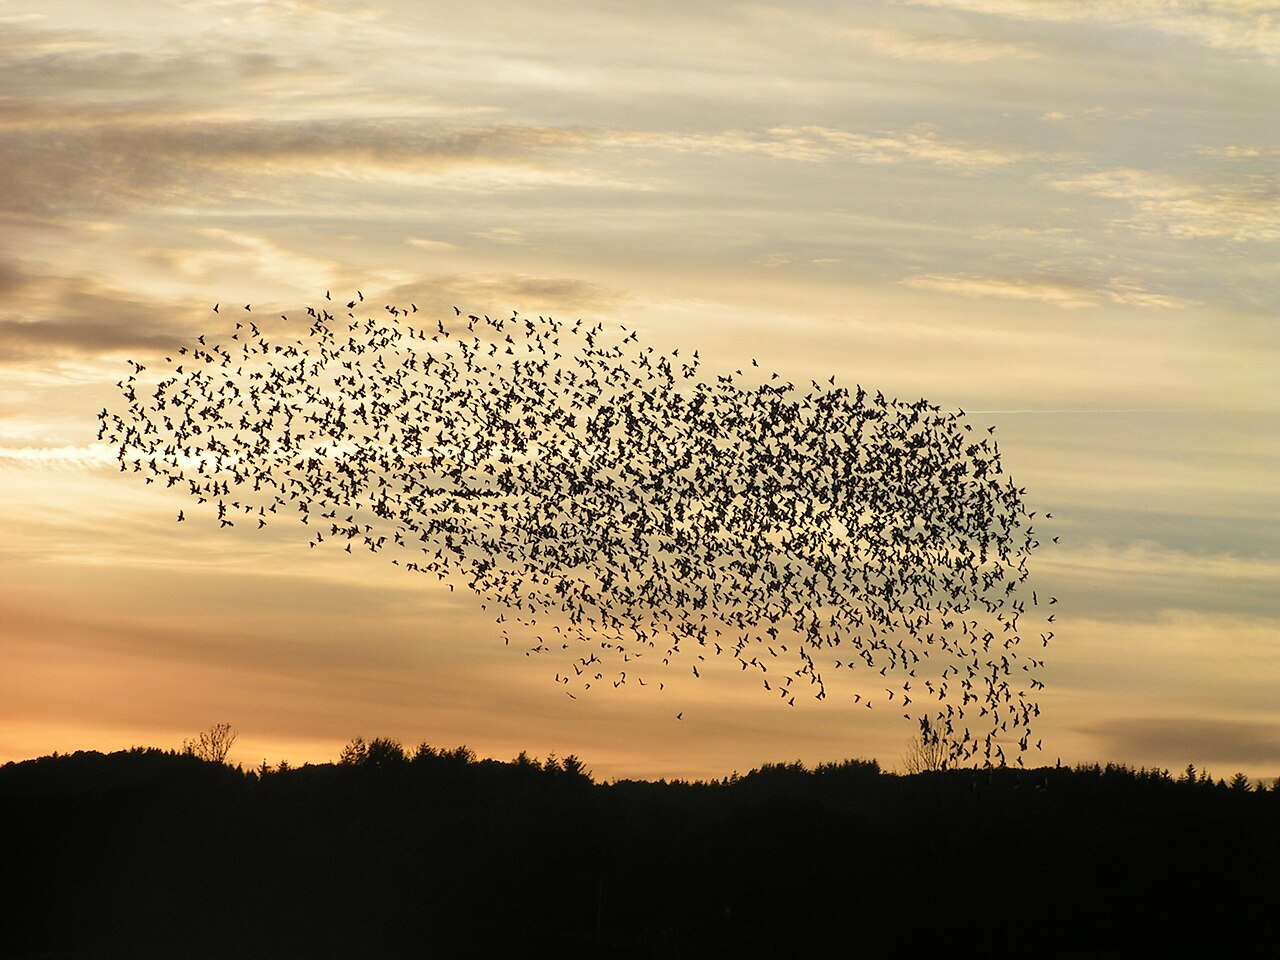
\includegraphics[width=\linewidth]{images/soa/murmuration.jpg}
\caption{Starlings over {\O}rns{\o}, Denmark}
\end{subfigure}\hspace{0.04\textwidth}
\begin{subfigure}[b]{0.40\textwidth}\centering
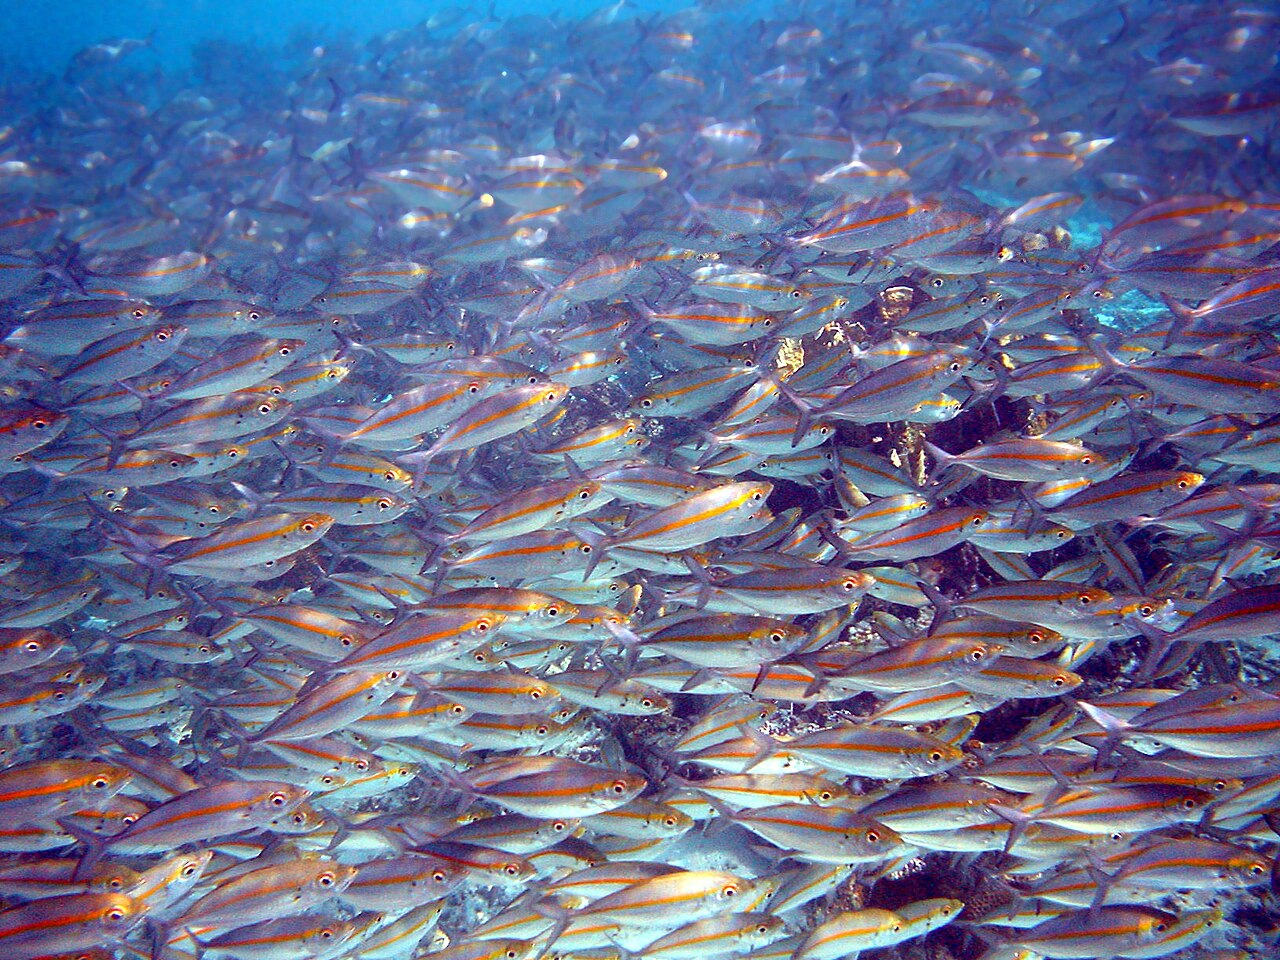
\includegraphics[width=\linewidth]{images/soa/fish_school.jpg}
\caption{A school of \emph{Pterocaesio chrysozona}}
\end{subfigure}
\caption[Collective motion in nature]{Collective motion in nature, with (a) starlings and (b) a fish school (photos by (a) Christoffer A. Rasmussen, public domain, and (b) Brocken Inaglory, \href{https://creativecommons.org/licenses/by-sa/3.0/}{CC~BY-SA~3.0}, via \href{https://commons.wikimedia.org/}{Wikimedia Commons}).}
\label{fig:soa-flocks}
\end{figure}

A boid is a vehicle that behaves as a point with a position $\mathbf{p}_i$ and a velocity $\mathbf{v}_i$, and it faces the direction of its velocity. At each update, it sees the set $N_i$ of flock members within a distance $r$ and a field of view $\theta$ measured from its direction of travel \citep{reynolds1987flocks}:
\begin{equation}
\boxed{N_i = \left\{\, j \neq i \;:\; \lVert \mathbf{p}_j - \mathbf{p}_i \rVert < r \;\wedge\; \angle\!\left(\mathbf{v}_i,\, \mathbf{p}_j - \mathbf{p}_i\right) < \tfrac{\theta}{2} \,\right\}}
\label{eq:neighbourhood}
\end{equation}
Three rules apply to this neighborhood, to avoid collision, to match velocity and to stay close (\cref{fig:boids-rules}). Reynolds expressed them in words, and the equations below are a typical way of writing them, each giving zero when $N_i$ is empty. Separation sums the vectors that point away from each neighbor, weighted by the inverse square of the distance, alignment matches the mean velocity of the neighbors, and cohesion pulls the boid toward their centroid:
\begin{equation}
\boxed{\mathbf{s}_i = \sum_{j \in N_i} \frac{\mathbf{p}_i - \mathbf{p}_j}{\lVert \mathbf{p}_i - \mathbf{p}_j \rVert^{2}}}
\label{eq:separation}
\end{equation}
\begin{equation}
\boxed{\mathbf{a}_i = \frac{1}{\lvert N_i \rvert} \sum_{j \in N_i} \mathbf{v}_j \;-\; \mathbf{v}_i}
\label{eq:alignment}
\end{equation}
\begin{equation}
\boxed{\mathbf{c}_i = \frac{1}{\lvert N_i \rvert} \sum_{j \in N_i} \mathbf{p}_j \;-\; \mathbf{p}_i}
\label{eq:cohesion}
\end{equation}
Separation is the only rule that keeps boids apart, and it is a weak constraint, because proximity only has a cost and boids can still overlap when other forces dominate. The centroid is local, so a flock can split around an obstacle and rejoin. Strangers on a street have no reason to stay together, so for pedestrians cohesion is generally low, present only within a group, and overridden by each person's destination.

\begin{figure}[H]
\centering
\begin{subfigure}[b]{0.31\textwidth}\centering
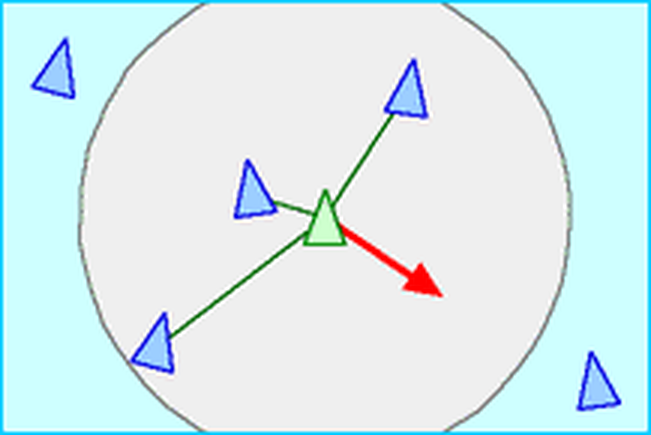
\includegraphics[width=\linewidth]{images/web/boids_rule_separation.png}
\caption{Separation}
\end{subfigure}\hfill
\begin{subfigure}[b]{0.31\textwidth}\centering
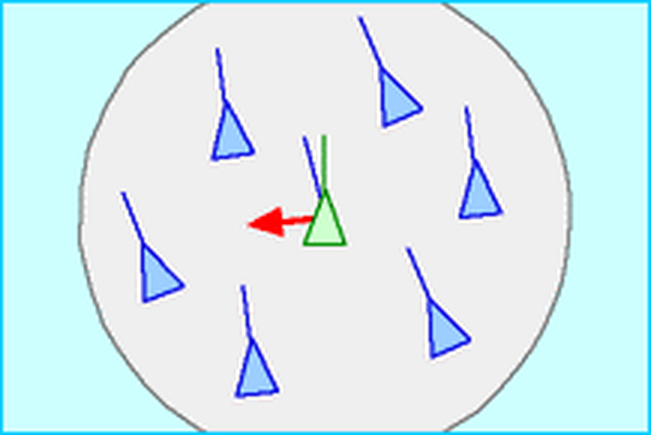
\includegraphics[width=\linewidth]{images/web/boids_rule_alignment.png}
\caption{Alignment}
\end{subfigure}\hfill
\begin{subfigure}[b]{0.31\textwidth}\centering
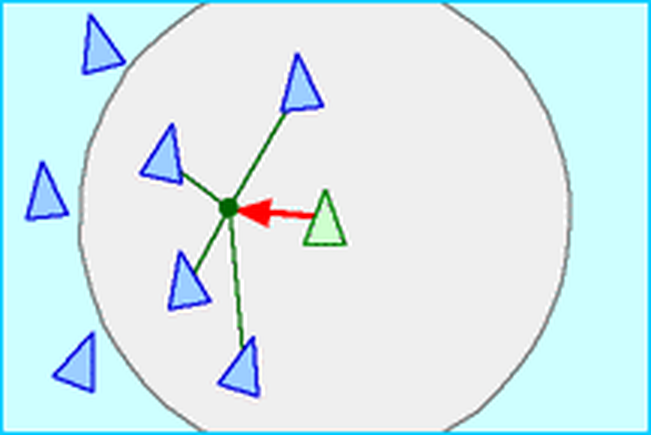
\includegraphics[width=\linewidth]{images/web/boids_rule_cohesion.png}
\caption{Cohesion}
\end{subfigure}
\caption[The three boids rules]{The three boids rules seen from the green boid, where the grey disc is its neighborhood and the red arrow is the steering that each rule produces (diagrams by Craig Reynolds, public domain, via \href{https://commons.wikimedia.org/}{Wikimedia Commons}).}
\label{fig:boids-rules}
\end{figure}

\citet{reynolds1999steering} built a library of steering behaviors on these rules and split movement into \emph{action selection} (choosing a goal), \emph{steering} (turning the goal into a desired change in motion) and \emph{locomotion} (the movement itself, \cref{fig:steering-pipeline}). In our design, authored rules take care of action selection and the boids-based navigation takes care of steering. The vehicle is a point mass $m$ with a maximum force $f_{\max}$ and a maximum speed $v_{\max}$:
\begin{equation}
\boxed{\mathbf{v} \leftarrow \operatorname{trunc}\!\left(\mathbf{v} + \frac{\operatorname{trunc}(\mathbf{f}, f_{\max})}{m}\,\Delta t,\; v_{\max}\right)\qquad
\mathbf{p} \leftarrow \mathbf{p} + \mathbf{v}\,\Delta t}
\label{eq:vehicle}
\end{equation}
Most behaviors compute a desired velocity $\mathbf{v}^{d}$ and set $\mathbf{f}$ to $\mathbf{v}^{d}$ minus $\mathbf{v}$, as in seek and flee, arrival, pursuit and evasion, wander, path following, obstacle avoidance with probes in front of the individual, and leader following.

\begin{figure}[H]
\centering
\begin{tikzpicture}[>=Latex, font=\footnotesize,
  box/.style={draw,rounded corners=2pt,align=center,inner sep=3pt},
  beh/.style={draw=cBlue!80!black,rounded corners=1pt,align=center,text width=2.6cm,minimum height=0.5cm,inner sep=2pt,fill=cBlue!12}]
\node[box,text width=2.3cm,minimum height=1.7cm,fill=cPurple!15,draw=cPurple!80!black] (sel) at (0,0) {\textbf{Action selection}\\[2pt]goals, plans, schedules};
\node[beh] (b1) at (3.9,1.75) {Seek / arrival};
\node[beh] (b2) at (3.9,1.05) {Path following};
\node[beh] (b3) at (3.9,0.35) {Obstacle avoidance};
\node[beh] (b4) at (3.9,-0.35) {Separation};
\node[beh] (b5) at (3.9,-1.05) {Alignment};
\node[beh] (b6) at (3.9,-1.75) {Cohesion};
\node[draw,dashed,rounded corners=3pt,fit=(b1)(b6),inner sep=4pt,label={[font=\footnotesize\bfseries]above:Steering behaviors}] (steer) {};
\node[box,text width=3.0cm,minimum height=1.7cm,fill=cOrange!15,draw=cOrange!80!black] (comb) at (8.0,0) {\textbf{Combination}\\[2pt]weighted sum $\sum_k w_k \mathbf{f}_k$\\or prioritized allocation};
\node[box,text width=2.4cm,minimum height=1.7cm,fill=cGreen!15,draw=cGreen!80!black] (loc) at (11.85,0) {\textbf{Locomotion}\\[2pt]truncate, integrate velocity and position, animate};
\node[box,text width=5.4cm,fill=cSky!15,draw=cSky!80!black] (per) at (8.6,-3.0) {\textbf{Perception}: neighbors within radius and field of view, obstacles, walls};
\draw[->,thick] (sel.east) -- node[above,font=\scriptsize]{targets} (sel.east -| steer.west);
\foreach \b in {b1,b2,b3,b4,b5,b6} \draw[->] (\b.east) -- (comb.west);
\draw[->,thick] (comb) -- node[above,font=\scriptsize]{$\mathbf{f}$} (loc);
\draw[->] (per.west) -| (steer.south);
\draw[->,dashed] (loc.south) |- node[pos=0.25,right,font=\scriptsize,align=left]{new position\\and velocity} (per.east);
\end{tikzpicture}
\caption[Steering between action selection and locomotion]{Steering behaviors between action selection and locomotion, after \citet{reynolds1999steering}.}
\label{fig:steering-pipeline}
\end{figure}

\subsection{Combining Behaviors}\label{combo}

A pedestrian that follows a path must also keep clear of other pedestrians and of walls, and the weighted sum is the simplest way of combining the forces, as \citet{reynolds1999steering} noted:
\begin{equation}
\boxed{\mathbf{f} = \operatorname{trunc}\!\left(\sum_{k} w_k\,\mathbf{f}_k,\; f_{\max}\right)}
\label{eq:weighted}
\end{equation}
It is cheap and gives smooth motion, but opposing forces can cancel each other out and leave the character stuck, a small force can hide a larger one, and weights that work in one situation may fail in another \citep{millington2019ai}. The alternative is priority, as in Reynolds' prioritized acceleration allocation, where requests fill an accumulator in order of priority until it reaches its capacity, and textbooks also blend within priority groups \citep{millington2019ai}. Many systems, ours included, use priority between layers and blending within a layer. Extensions of the original rules add forces for leadership changes \citep{hartman2006autonomous}, fear signals that reach animals which cannot see the threat \citep{delgadomata2007fear} and escape, which in a building means competing for exits, where pushing makes everyone slower \citep{helbing2000simulating}.

\subsection{Cost of Neighbor Search}\label{sub:complexity}

In each frame, each boid evaluates \cref{eq:neighbourhood,eq:separation,eq:alignment,eq:cohesion} from a snapshot of the previous state, combines the forces with \cref{eq:weighted} and integrates them with \cref{eq:vehicle}, so the result does not depend on the order of updates and the algorithm parallelizes well. A direct search performs $O(n^2)$ distance tests per frame, which is the main bottleneck with thousands of individuals. The usual remedy is a uniform grid whose cells are at least as large as the perception radius, so that a query visits only the neighboring cells and its cost depends on the local density \citep{ericson2004realtime,reynolds2006big}. Hierarchical structures such as k-d trees \citep{bentley1975multidimensional} adapt better to clustered individuals but cost more to rebuild every frame (\cref{fig:soa-kdtree}). General-purpose \gls{gpu} computation suits boids, because each individual only reads the previous state \citep{owens2007survey,joselli2009neighborhood}, and approximate or capped neighbor sets reduce the cost further \citep{joselli2009neighborhood,silva2009boids}, although these change the model and should be reported.

\begin{figure}[H]
\centering
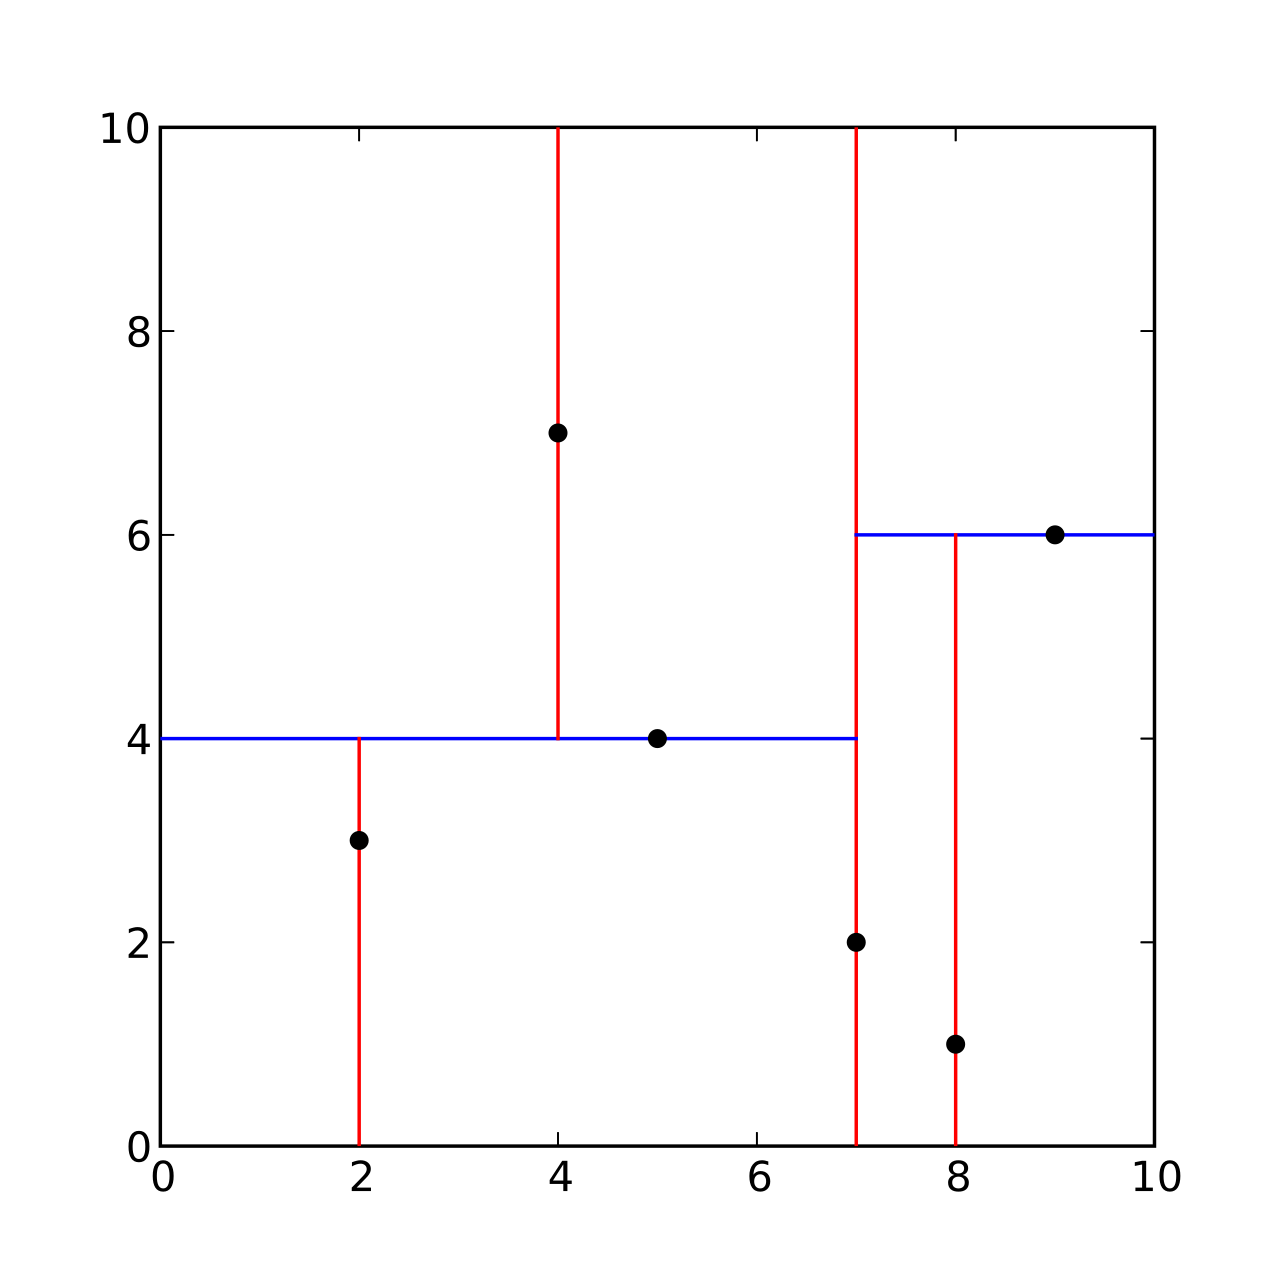
\includegraphics[width=0.30\textwidth]{images/soa/kdtree.png}
\caption[A two-dimensional k-d tree]{A two-dimensional k-d tree for seven points (image by KiwiSunset, English Wikipedia, \href{https://creativecommons.org/licenses/by-sa/3.0/}{CC~BY-SA~3.0}, via \href{https://commons.wikimedia.org/}{Wikimedia Commons}).}
\label{fig:soa-kdtree}
\end{figure}

\section{Agent-Based Modeling}\label{sec:ABM}

An \gls{abm} represents a system as a collection of autonomous individuals, each of which assesses its own situation and acts according to a set of rules \citep{bonabeau2002agent}, and boids are a classic example. \citet{macal2010tutorial} describe a model through individuals with attributes and behaviors, their interactions and their environment. Toolkits such as NetLogo \citep{wilensky1999netlogo}, MASON \citep{luke2005mason} and Repast Simphony \citep{north2013complex} target general modeling rather than animated characters on navigation meshes, which is one reason why interactive crowds are built inside game engines. Outcomes are usually emergent, as with lane formation in counter-flows \citep{helbing2005self}, so modelers observe them over many seeded runs and summarize them statistically. The \acrshort{odd} protocol \citep{grimm2006standard,grimm2020odd} also asks modelers to report hidden design decisions, such as the order of updates and how time advances.

A population can be studied top-down through aggregate equations, as when \citet{hughes2002continuum} treats the crowd as a fluid moving down a potential, or bottom-up through individuals. \citet{vandykeparunak1998agent} found that agent-based models suit systems with discrete decision makers, each with its own history, while equation-based models suit systems that aggregates describe well. Corridor flow obeys aggregate relations, but whether a worker finds a free desk depends on what other people did that morning, which is the kind of question this thesis addresses.

\section{Action Selection and Crowd Models}\label{auto}

A \gls{fsm} has one state at a time and changes state when a condition is met, so the number of transitions grows quickly as states are added \citep{millington2019ai}. Behavior trees, popularized by Halo~2 \citep{isla2005handling}, compose sequences and selectors from leaves and are more modular and reactive \citep{millington2019ai,colledanchise2018behavior} (\cref{fig:soa-bt}). Goal-oriented action planning searches for actions whose preconditions and effects reach a goal \citep{orkin2006three}, and utility-based selection scores the options \citep{graham2019introduction}. These describe how to behave rather than when, so time of day and resource availability must be modeled separately. Other work moves knowledge into the environment, with smart objects that describe how they are used \citep{kallmann1999modeling}, objects in The Sims that advertise how much they satisfy a motivation \citep{forbus2001notes} and behaviors attached to regions \citep{sung2004scalable}, and our stations derive from these ideas. Data-driven and learned approaches reuse recorded trajectories \citep{lerner2007crowds} or train individual policies \citep{juliani2018unity}, such as collision avoidance \citep{lee2018crowd}, but they address local motion, and a user who must state who arrives when gains little from a policy that hides its assumptions in weights.

\begin{figure}[H]
\centering
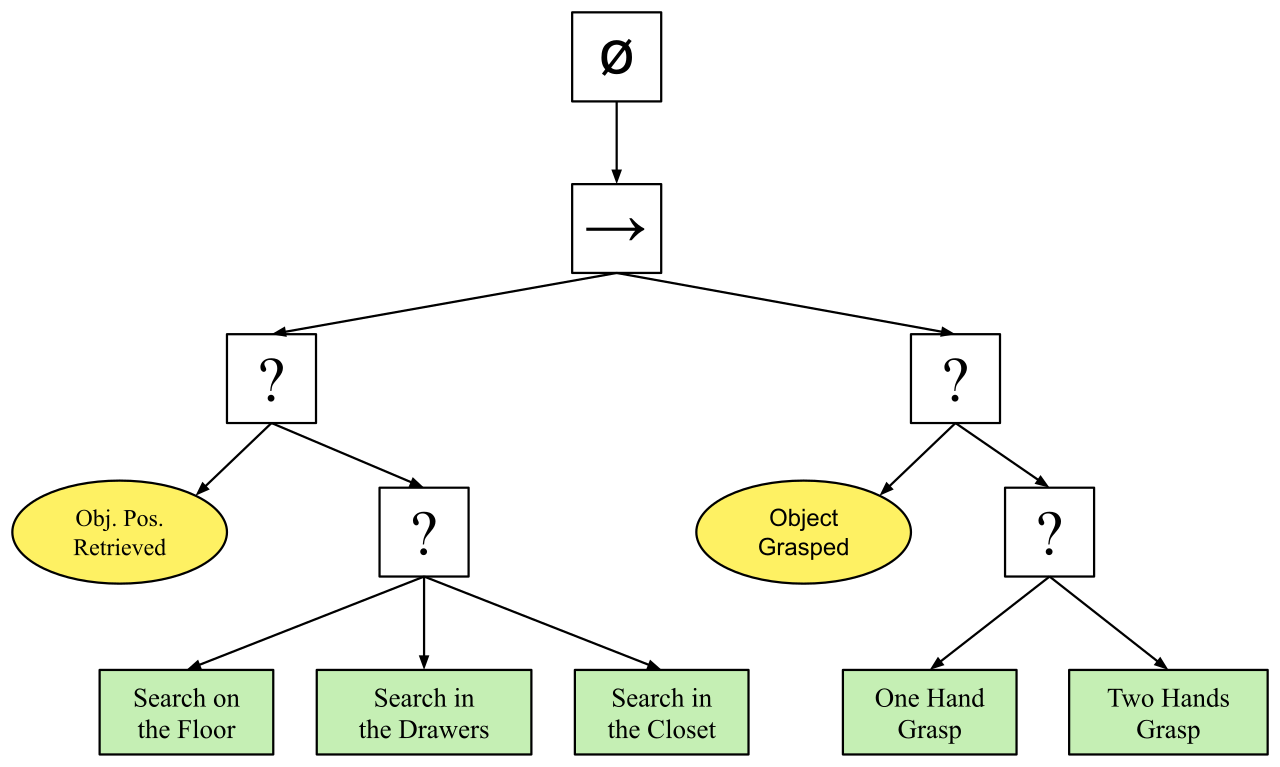
\includegraphics[width=0.45\textwidth]{images/soa/behaviour_tree.png}
\caption[A behavior tree]{A behavior tree for a robot that finds and grasps an object \citep{colledanchise2018behavior} (diagram by Aliekor, English Wikipedia, \href{https://creativecommons.org/licenses/by-sa/3.0/}{CC~BY-SA~3.0}, via \href{https://commons.wikimedia.org/}{Wikimedia Commons}).}
\label{fig:soa-bt}
\end{figure}

Game engines now provide much of this infrastructure, and we draw on the current Unreal Engine documentation for its concepts, although the implementation uses version~5.4. The Navigation System builds a navigation mesh with Recast and answers path queries \citep{epicgames2026navigation,mononen2009recast} (\cref{fig:soa-navmesh}), with \gls{rvo} avoidance in the Character Movement component and adaptive \gls{rvo} sampling in the Detour Crowd manager \citep{epicgames2026avoidance}. Behavior trees and State Trees support decisions \citep{epicgames2026statetree}, Smart Objects have slots that characters claim and release \citep{epicgames2026smartobjects}, and Mass Entity, the Mass Gameplay plugins and ZoneGraph lanes support large numbers of characters \citep{epicgames2026massentity,epicgames2026massgameplay,epicgames2026zonegraph}. Who does what and when, the order of waiting and the service time are all left to the developer. Unlike Smart Objects, which let characters claim and release slots, our stations add a capacity, a first-come, first-served queue, a timed service and ordered multi-stage use, and our schedules add the timing and deferral rules that decide when each request is made. Menge makes goal selection, planning and local avoidance pluggable components \citep{curtis2016menge}, which is also our motivation at the boundary between activity and movement.

\begin{figure}[H]
\centering
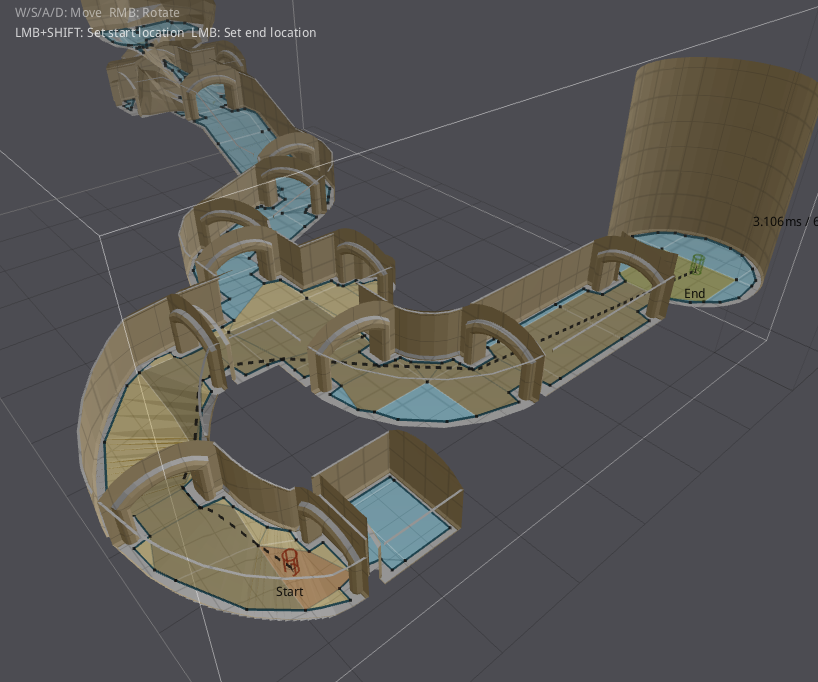
\includegraphics[width=0.42\textwidth]{images/soa/recast_navmesh_crop.png}
\caption[A navigation mesh built by Recast]{A navigation mesh built by Recast, with a path found by Detour (cropped screenshot of RecastDemo, Recast \& Detour \textcopyright{}~2009 Mikko Mononen, zlib license, \href{https://github.com/recastnavigation/recastnavigation}{github.com/recastnavigation}).}
\label{fig:soa-navmesh}
\end{figure}

General references on crowd simulation are \citet{thalmann2013crowd}, \citet{pelechano2008virtual} and \citet{kapadia2016virtual}, with a history by \citet{musse2021history}, and the motion models below all take their targets from an action selection layer (\cref{fig:model-taxonomy}). Macroscopic models evolve a density field over a cost potential \citep{hughes2002continuum,treuille2006continuum}, and cellular automata with floor fields \citep{burstedde2001simulation,kirchner2002simulation} are fast but too coarse for animated motion (\cref{fig:soa-ca}). Microscopic models compute motion per pedestrian with social forces \citep{helbing1995social}, HiDAC \mbox{\citep{pelechano2007controlling}}, reciprocal velocity obstacles and \gls{orca} \citep{vandenberg2008reciprocal,vandenberg2011reciprocal} (\cref{fig:soa-vo}), a time-to-collision law \citep{karamouzas2014universal} or vision-based heuristics \citep{moussaid2011simple}, as surveyed by \citet{vantoll2021algorithms}. Force-based models and boids only penalize overlap, velocity obstacle models avoid it under their own assumptions, and the walker experiments of \citet{pettre2009experiment} show that both people share the avoidance. None of these models provides targets, so the authoring problem would be the same with any of them.

\begin{figure}[H]
\centering
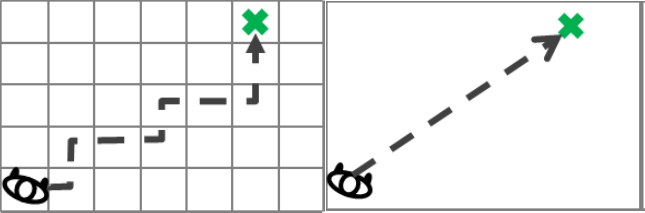
\includegraphics[width=0.5\textwidth]{images/soa/grid_vs_continuous.png}
\caption[Movement on a grid and in continuous space]{Movement on a grid of cells, on the left, and in continuous space, on the right (diagram by Angelika Kneidl, \href{https://creativecommons.org/licenses/by-sa/4.0/}{CC~BY-SA~4.0}, via \href{https://commons.wikimedia.org/}{Wikimedia Commons}).}
\label{fig:soa-ca}
\end{figure}

\begin{figure}[H]
\centering
\begin{tikzpicture}[>=Latex, font=\footnotesize, scale=0.95,
  lab/.style={fill=white,inner sep=1.5pt,align=center}]
% cone of velocities of A that hit B: apex at A + v_B, edges parallel to the tangents from A to the widened B
\fill[cVerm!15] (-1.2,1.2) -- (7.674,2.7) -- (7.674,-0.3) -- cycle;
\draw[cVerm!80!black] (-1.2,1.2) -- (7.674,2.7);
\draw[cVerm!80!black] (-1.2,1.2) -- (7.674,-0.3);
% the two people
\draw[cOrange!80!black,dashed] (6,0) circle (1.0);
\filldraw[fill=cOrange!40,draw=cOrange!80!black] (0,0) circle (0.45) node {$A$};
\filldraw[fill=cOrange!40,draw=cOrange!80!black] (6,0) circle (0.55) node {$B$};
\node[lab,text=black!70] at (6,-1.6) {$B$ widened by\\the radius of $A$};
% B's velocity, and the same vector placed at A, which moves the apex of the cone
\draw[->,very thick,cBlue] (6,0) -- (4.8,1.2);
\node[lab,text=cBlue!80!black,anchor=west] at (6.75,1.05) {velocity of $B$};
\draw[->,thick,cBlue,densely dotted] (0,0) -- (-1.2,1.2) node[lab,above left=0pt]{velocity of $B$,\\placed at $A$};
% two candidate velocities of A
\draw[->,very thick,cVerm] (0,0) -- (3.0,1.2) node[lab,above=2pt]{collides};
\draw[->,very thick,cGreen!80!black] (0,0) -- (2.6,-0.9) node[lab,right=2pt]{stays clear};
\node[lab,text=cVerm!80!black] at (4.3,3.25) {velocity obstacle: the velocities of $A$\\that lead to a collision with $B$};
\draw[->,cVerm!80!black] (4.3,2.8) -- (4.3,2.05);
\end{tikzpicture}
\caption[A velocity obstacle]{A velocity obstacle, where every velocity of $A$ that ends inside the shaded cone leads to a collision with $B$ if both keep moving, so velocity obstacle models choose a velocity outside it \citep{vandenberg2008reciprocal}.}
\label{fig:soa-vo}
\end{figure}

\begin{figure}[H]
\centering
\begin{tikzpicture}[>=Latex, font=\footnotesize,
  cat/.style={draw,rounded corners=2pt,align=center,inner sep=3pt,fill=black!8,minimum width=2.6cm},
  leaf/.style={draw,rounded corners=1pt,align=left,inner sep=3pt},
  edge/.style={->}]
\node[draw=cPurple!80!black,dashed,rounded corners=2pt,align=center,text width=9cm,inner sep=4pt,fill=cPurple!12] (sel) at (0,1.5) {\textbf{Action selection}: goals, plans, schedules, smart objects (where and why individuals move)};
\node[cat] (root) at (0,0) {\textbf{Crowd motion models}};
\draw[edge,thick] (sel) -- node[right,font=\scriptsize]{targets} (root);
\node[cat,fill=cBlue!18,draw=cBlue!80!black] (macro) at (-5.6,-1.4) {Macroscopic};
\node[cat,fill=cOrange!20,draw=cOrange!80!black] (micro) at (0,-1.4) {Microscopic};
\node[cat,fill=cGreen!18,draw=cGreen!80!black] (hyb) at (5.6,-1.4) {Hybrid};
\draw[edge] (root.south) -- (macro.north);
\draw[edge] (root.south) -- (micro.north);
\draw[edge] (root.south) -- (hyb.north);
\node[cat,minimum width=2.2cm,fill=cOrange!10,draw=cOrange!80!black] (cont) at (-1.75,-2.7) {Continuous space};
\node[cat,minimum width=2.2cm,fill=cOrange!10,draw=cOrange!80!black] (disc) at (1.95,-2.7) {Discrete space};
\draw[edge] (micro.south) -- (cont.north);
\draw[edge] (micro.south) -- (disc.north);
\node[leaf,text width=3.1cm,anchor=north] (macroleaf) at (-5.6,-2.15) {Continuum and flow models over density and velocity fields \citep{hughes2002continuum,treuille2006continuum}};
\node[leaf,text width=3.3cm,anchor=north] (contleaf) at (-1.75,-3.25) {Rules: boids, steering\\Forces: social force, HiDAC\\Velocities: RVO, ORCA\\Anticipation and vision\\Data-driven and learned};
\node[leaf,text width=2.6cm,anchor=north] (discleaf) at (1.95,-3.25) {Cellular automata with floor fields \citep{burstedde2001simulation,kirchner2002simulation}};
\node[leaf,text width=3.1cm,anchor=north] (hybleaf) at (5.6,-2.15) {Microscopic rules for individuals under macroscopic rules for groups \citep{Agent}};
\draw[edge] (macro) -- (macroleaf);
\draw[edge] (cont) -- (contleaf);
\draw[edge] (disc) -- (discleaf);
\draw[edge] (hyb) -- (hybleaf);
\end{tikzpicture}
\caption[A taxonomy of crowd motion models]{A taxonomy of crowd motion models.}
\label{fig:model-taxonomy}
\end{figure}

\section{Purposeful Populations and Shared Resources}\label{sec:soa-purpose}

Systems that aim for believable populations combine decision-making with crowd motion, usually in layers. \citet{hoogendoorn2004pedestrian} distinguish a strategic level (choosing and scheduling activities), a tactical level (areas and routes) and an operational level (walking), and \citet{musse2001hierarchical} and Menge \citep{curtis2016menge} layer control in a similar way. In our system, schedules and stations act at the strategic and tactical levels and the boid-guided paths at the operational level.

Several systems give a population purpose through activities: needs-driven travelers in Pennsylvania Station \citep{shao2007autonomous}, an activity-driven population \citep{paris2009activity}, roles and schedules \citep{pelechano2008virtual}, CAROSA's roles, schedules and parameterized actions \citep{allbeck2010carosa}, transit trips generated for a crowd simulator \citep{ricks2020generation} and MATSim's daily activity plans, which are improved through repeated simulation \citep{horni2016matsim}, and \cref{tab:activity-systems} compares them with this thesis. Authored time-of-day schedules are also common in commercial games, as role-playing games such as The Elder Scrolls IV: Oblivion \citep{bethesda2006oblivion} and V: Skyrim \citep{bethesda2011skyrim} give their non-player characters daily packages with time windows. Farming games such as Stardew Valley \citep{concernedape2016stardew} read the schedules of their characters from data files. Pedestrian simulators for building design, such as MassMotion \citep{oasys2026massmotion}, Pathfinder \citep{thunderhead2026pathfinder}, Vadere \citep{kleinmeier2019vadere} and JuPedSim \citep{jupedsim2026}, model services, waiting areas and queues. Neither group combines authored schedules with capacity-limited resources and boids steering inside a general game engine, but both show that schedules and queues on their own are not new, so our contribution lies in their combination and in the timing semantics of \cref{chap:problem}.

\citet{Agent}\label{sec:soa-saeed} combine microscopic rules for pedestrians, who have attributes such as age, velocity and energy, with macroscopic rules for subgroups that share an intention over several goal points. They sum the steering, obstacle and pedestrian-avoidance forces into one, combine flocking with pathfinding over a navigation mesh \citep{hart1968formal,snook2000simplified} and first test their components in a simple scenario, as the scenario suites of SteerBench \citep{singh2009steerbench} and RiMEA \citep{rimea2025guideline} also do. It is the published work closest to our movement design, while \citet{shao2007autonomous} and CAROSA \citep{allbeck2010carosa} are closer on timing and resources. As we read it, it addresses motion, with goals and group intentions but no timed schedules or capacity constraints. In their summed forces the flock can pull individuals off their route, while in our hybrid boids the path dominates and steering can only turn the heading by a bounded amount.

\begin{table}[H]
\centering
\footnotesize
\begin{tabularx}{\textwidth}{|>{\raggedright\arraybackslash}p{2.5cm}|>{\raggedright\arraybackslash}X|>{\raggedright\arraybackslash}X|>{\raggedright\arraybackslash}X|>{\raggedright\arraybackslash}X|}
\hline
\rowcolor{headgray}\textbf{Work} & \textbf{Source of purpose} & \textbf{Timing of activities} & \textbf{Shared resources} & \textbf{Local motion} \\
\hline
\citet{shao2007autonomous} & Internal needs and goals in a cognitive layer & Driven by needs and events & Ticket queues in the station & Reactive behaviors with perception \\ \hline
\citet{paris2009activity} & Cognitive, goal-oriented activities & Activity-driven & Not a focus & Not a focus \\ \hline
CAROSA \citep{allbeck2010carosa} & Roles and parameterized actions & Authored schedules & Not a focus & Not a focus \\ \hline
\citet{ricks2020generation} & Generated trips in a transit facility & Generated arrival and destination times & Not a focus & Separate crowd simulator \\ \hline
MATSim \citep{horni2016matsim} & Daily activity plans & Activity times in plans, improved by replanning & Not at pedestrian level & Network-level trips, no steering \\ \hline
Menge \citep{curtis2016menge} & Finite-state goal selection & Not a focus & Not a focus & Replaceable local-avoidance component \\ \hline
Unreal Engine tools \citep{epicgames2026statetree,epicgames2026smartobjects} & Behavior trees or State Tree written by the developer & Developer's own logic & Smart Object slots claimed and released & Navigation mesh paths with avoidance \\ \hline
\citet{Agent} & Group intentions over several goal points & Not a focus & Not a focus & Combined steering forces \\ \hline
This thesis & Authored timed rules in readable files & Rules eligible from a time, deferred while the person is busy & Stations with capacity, \glsentryshort{fifo} queue and service time & Boids bounded around navigation mesh paths \\ \hline
\end{tabularx}
\caption[Systems that give simulated populations purpose]{Systems that give simulated populations purpose, where ``not a focus'' means that the work does not present that aspect.}
\label{tab:activity-systems}
\end{table}

Once individuals need resources, waiting is part of the outcome. In Kendall's notation, a counter with $c$ places is an M/M/$c$ or, without statistical assumptions, a G/G/$c$ queue \citep{kendall1953stochastic}. Little's law ($L = \lambda W$) links the mean number in a system to the arrival rate and the mean time spent in it \citep{little1961proof}, and waiting grows sharply as the utilization $\rho = \lambda/(c\mu)$ approaches 1 \citep{shortle2018fundamentals}. These results assume steady arrivals, but scheduled demand comes in waves and late starts push later arrivals, so we measure queues rather than calculate them, as discrete-event simulation does \citep{law2015simulation}. Commercial pedestrian tools such as the AnyLogic Pedestrian Library combine walking with services, waiting areas and queues \citep{anylogic2026pedestrian}, but they model a facility, while our setting is a game-engine population with authored schedules. Physical space is a second dimension, as Fruin's levels of service rate areas by space per pedestrian \citep{fruin1971pedestrian}, Weidmann relates walking speed (about 1.34~m/s when free) to density \citep{weidmann1993transporttechnik} and HiDAC models queueing physically \mbox{\citep{pelechano2007controlling}}. A queue kept as an ordered list ignores these effects, which makes timing analysis much easier but limits the claims that can be made about crowding.

For a purposeful crowd, evacuation and validation remain open. \citet{schadschneider2009evacuation} review evacuation research, whose simulations reproduce clogging and the faster-is-slower effect \citep{helbing2000simulating}, and \citet{kuligowski2010review} compare the models in use. In an activity-driven population, individuals are queueing, being served or walking when the alarm sounds, and where they were shapes how they leave. Validation compares a simulation with real behavior, through fundamental diagrams for single files \citep{seyfried2005fundamental} and for corridors and T-junctions \citep{zhang2011transitions}, pairwise avoidance against motion capture \citep{pettre2009experiment}, stop-and-go waves \citep{lemercier2012realistic}, lane formation and bottleneck oscillations \citep{helbing2005self}, and experiments in which people steer avatars in a virtual environment \citep{moussaid2016crowd} (\cref{fig:soa-bottleneck}). SteerBench \citep{singh2009steerbench}, the RiMEA test cases \citep{rimea2025guideline} and ISO~20414 \citep{iso2020evacuation} formalize test scenarios and protocols. Most game-engine crowds, ours included, are not validated to that standard, so we make no claim of behavioral validity, but the thesis provides the instrumentation that validation would require.

\begin{figure}[H]
\centering
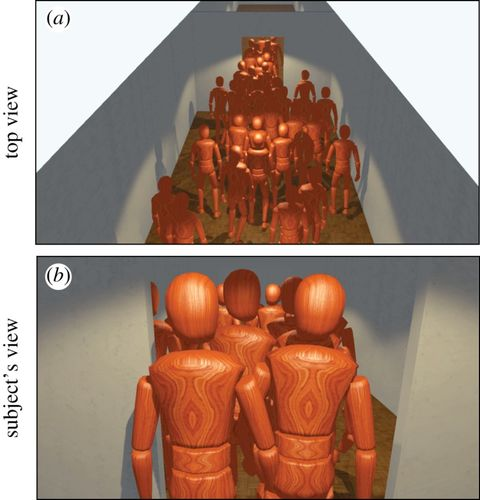
\includegraphics[width=0.30\textwidth]{images/soa/bottleneck_experiment.jpg}
\caption[A bottleneck experiment in a virtual environment]{A bottleneck evacuation experiment in a virtual environment, seen (a) from above and (b) by one participant (Figure~1 of \citet{moussaid2016crowd}, \href{https://creativecommons.org/licenses/by/4.0/}{CC~BY~4.0}, via \href{https://commons.wikimedia.org/}{Wikimedia Commons}).}
\label{fig:soa-bottleneck}
\end{figure}

\section{Discussion}\label{sec:soa-discussion}

The work reviewed covers each element of our problem but not their combination. Boids and steering give cheap and readable motion \citep{reynolds1999steering,reynolds2006big}, crowd models give more realistic motion \citep{vantoll2021algorithms}, the engine offers decisions with navigation and object reservation \citep{epicgames2026statetree,epicgames2026smartobjects}, timed purpose comes from activity-driven crowds \citep{shao2007autonomous,allbeck2010carosa,horni2016matsim}, and queueing theory deals with contention \citep{little1961proof}.

What is missing is the combination of these elements in one game-engine system, in which the user writes out timed activities for a reusable boids population and the capacity-limited shared resources, rather than the user, determine when each activity actually takes place. Each system in \cref{tab:activity-systems} lacks one of these elements, because the research systems have no capacity, queues or engine, the engine tools leave scheduling and queueing to the developer, and \citet{Agent} have goals but no timing or contention. The next chapter turns that gap into a description of the behavior we want and its functional requirements.
